\documentclass[a4paper]{article}
\usepackage[utf8]{inputenc}
\usepackage[frenchb]{babel}
\usepackage[T1]{fontenc}
\usepackage{graphicx}
\usepackage{fullpage}
\usepackage{hyperref}
\usepackage{listings}
\usepackage{color}
\usepackage[noend]{algpseudocode}
\usepackage{algorithm}
\usepackage{amsmath,amssymb, amsthm}
\usepackage{xspace}
\usepackage{subfig, tikz, calc}
\usetikzlibrary{trees, arrows, positioning, shapes}

\tikzset{
    orangenode/.style={rectangle,draw=black, top color=orange!40, bottom color=orange!40,very thick, inner sep=1em, minimum size=3em, text centered},
    bluenode/.style={rectangle,draw=black, top color=blue!40, bottom color=blue!40,very thick, inner sep=1em, minimum size=3em, text centered},
    myarrow/.style={->, >=latex', shorten >=1pt, thick},
    mylabel/.style={text width=7em, text centered},
    mydot/.style={draw, shape=circle, fill=black}
}

\def\sparql{\textsc{SPARQL}\xspace}
\def\fedra{\textsc{Fedra}\xspace}
\def\fedx{\textsc{FedX}\xspace}
\def\fexOpt{\textsc{FedXOpt}\xspace}
\def\peneloop{\textsc{PeNeLoop}\xspace}

\newcommand{\parallelLink}[1]{Version avec requêtes parallélisées \href{#1}{disponible ici}.}

\newtheorem{hypo}{Hypothèse}

\hypersetup{
    colorlinks=true,
    linkcolor=blue,
    urlcolor=blue
}

\title{\peneloop : Parallelizing federated \sparql query using replicated fragments\\Rapport de travail}
\author{Thomas \textsc{Minier}}
\date{Mai-Juillet 2016}

\begin{document}

\maketitle

\tableofcontents

\newpage

%--------------------------
\section{Introduction}

%--------------------------
\subsection{Contexte et motivation}

Dans le domaine des bases de données distribuées, une pratique courante pour accroître la disponibilité des données est de les répliquer. Elle consiste à diviser le schéma de stockage des données en plusieurs sous-schémas, appelés \textit{fragments}, puis à répartir de multiples copies de chacun de ses fragments sur différents serveurs, appelés \textit{répliques}. Chaque fragment est ainsi disponible à plusieurs endroits et si l'un des serveurs venait à être inaccessible, les données seraient toujours disponibles auprès des autres répliques.

Cependant, les moteurs de requêtes \sparql fédérées actuels \cite{schwarte2011fedx,acosta2011anapsid} gèrent très mal la réplication des données. Ils ne sont pas capables de sélectionner les sources pertinentes d'une requête en détectant lesquels sont des répliques afin de les éliminer de la sélection. Ils effectuent donc les mêmes requêtes sur des serveurs qui contiennent les mêmes données et, par conséquent, transfèrent des données dupliquées superflues qui ralentissent les performances générales du moteur de requête. \fedra \cite{montoya2014fedra} propose un algorithme de sélection de sources capable de résoudre ces problèmes. En regroupant les répliques entre elles, il est capable de sélectionner l'ensemble minimal de sources nécessaire pour répondre à une requête. Cela permet une nette amélioration du temps d'exécution et du nombre de résultats transférés lors de l'exécution de requêtes \sparql fédérées dans un contexte où les données sont répliquées. La figure \ref{fig:source_selection_movies} montre un exemple de sélection de sources effectuée par \fedra pour la requête de la figure \ref{query:movies}.

\begin{figure}[h]
    \centering
    \subfloat[Requête exécutée sur la fédération $E1,E2,E3,E4$]{
        \lstinputlisting[basicstyle=\scriptsize\sffamily,language=sparql,numbers=none,frame=none,columns=fixed,extendedchars=true,breaklines=true,showstringspaces=false]{sparql/queryExample.txt}
         \label{query:movies}
     }
    \subfloat[Fragments (F) \& Sélection de source par \fedra]{
    \label{fig:source_selection_movies}
        \begin{scriptsize}
            \begin{tabular}{|c|c|c|c|} \hline
                Triple pattern & F & Endpoints & Sélection de sources \\
                \hline
                tp1 & f3 & E4 & $\{ \{ E4 \} \}$ \\
                \hline
                & f1 & E1 &  \\
                \cline{3-3}
                tp2 &  & E2 & $\{\{ E1,E2 \} , E3 \}$ \\
                 \cline{2-3}
                 & f2 & E3 &  \\
                \hline
            \end{tabular}
        \end{scriptsize}
    }
    \caption{Exemple de sélection de sources effectuée par \fedra pour une requête SPARQL fédérée}
\end{figure}

Néanmoins, \fedra ne tire pas parti des informations qu'il récupère concernant les répliques parmi les sources qu'il sélectionne. En les utilisant, il est possible d'améliorer de manière plus poussée l'exécution des requêtes grâce à la parallélisation. En effet, si pour une source donnée, on connaît les autres sources qui contiennent les mêmes fragments de données, on peut distribuer l'exécution des requêtes effectuées sur cette source à l'échelle de toutes les répliques. Ce faisant, nous pouvons améliorer le temps d'exécution des requêtes et la répartition de la charge sur les différentes sources de la fédération.

%--------------------------
\subsection{Contribution}

Notre problématique est donc de trouver une approche pour paralléliser l'exécution des requêtes \sparql fédérées dans un contexte de données répliquées. Pour ce faire, nous proposons \peneloop, un algorithme pour tirer parti des informations sur les répliques collectées par \fedra et améliorer les performances des requêtes \sparql fédérées en présence de données répliquées. Nous concentrerons notre travail sur la parallélisation de l'opérateur de jointure. Des algorithmes pour effectuer des jointures parallélisées dans un contexte de réplication ont déjà été évoqués dans la littérature \cite{ozsu2011principles}. Nous nous baserons sur l'algorithme du \textit{Parallel Nested Loop Join} pour notre travail, car il peut être appliqué sans connaître d'informations particulières sur la cardinalité des triples patterns impliqués dans une jointure. Or, dans notre contexte, nous nous basons sur \fedra pour récupérer les données sur la sélection des sources, et ce dernier travaille sans aucune informations sur la cardinalité des triples patterns évalués.

Nous présenterons d'abord le principe du Parallel Nested Loop Join dans le cadre d'une requête \sparql, puis nous étudierons deux approches pour le paralléliser. La première sera modélisée comme un problème de Bin Packing où l'on parallélise l'exécution des jointures elles-mêmes. La deuxième poussera la parallélisation plus loin, en se plaçant dans une architecture de type pipeline, où les jointures seront exécutées en parallèle entre elles. Pour chaque approche, nous étudierons d'abord l'aspect algorithmique, puis nous mènerons une étude expérimentale pour évaluer son efficacité. Nous présenterons également la configuration expéirmentale utilisée pour nos expérimentations. Enfin, nous conclurons pour déterminer quelle approche est la plus intéressante et la plus efficace pour répondre à notre problématique.

%--------------------------
\section{Hypothèses}

Voici les différentes hypothèses que nous avons émises lors de notre travail.

\begin{hypo}\label{hypo:localityANDparallel}
Soit une fédération $F$ contenant $N$ serveurs où les données ont été réparties en fragments parmi les $N$ serveurs. Soit une requête $R$ composée de $M$ triples patterns exécutée sur $F$. Chaque triple pattern de $R$ peut être soit localisé, soit parallélisé, ou aucun des deux. De plus, chaque groupe de triples patterns localisés peut être parallélisé ou non. 

Quelque soit le contexte, la capacité d'un triple pattern à être localisé ou parallélisé dépend du schéma de répartition des fragments parmi $F$.
\end{hypo}

\begin{hypo}\label{hypo:localityVSparallel}
Soit une fédération $F$ contenant $N$ serveurs où les données ont été réparties en fragments parmi les $N$ serveurs. Soit une requête $R$ composée de $M$ triples patterns exécutée sur $F$. Plus $N$ augmente, plus le nombre de triples patterns de $R$ qui sont localisées va diminuer et plus le nombre de triples patterns de $R$ qui sont parallélisés va augmenter. 
\end{hypo}

\begin{hypo}\label{hypo:stableTuples}
Soit une requête $R$ contenant une jointure entre deux triples patterns $tp_1, tp_2$ effectuée selon l'algorithme Parallel Nested Loop Join. Soit un ensemble de serveurs $E$ contenant les sources pertinentes de $tp_2$. L'exécution des requêtes de l'inner loop sur un serveur de $E$ transfère le même nombre de résultats intermédiaires que l'exécution des mêmes requêtes réparties sur l'ensemble des serveurs de $E$.
\end{hypo}

%--------------------------
\section{Parallel Nested Loop Join appliquée à une requête \sparql}

\subsection{Principes de base}

Considérons une jointure entre deux triples patterns $tp_1$ et $tp_2$ effectuée selon l'algorithme Parallel Nested Loop Join, et les sources $s_1$ et $s_2$ qui contiennent respectivement les données correspondant à $tp_1$ et à $tp_2$. L'algorithme va commencer par exécuter une première boucle sur les données de $s_1$ appelée \textbf{l'outer loop}. Pour chaque binding $b_n$ trouvé dans $s_1$ qui satisfait le pattern $tp_1$, l'algorithme va effectuer une autre boucle sur les données de $s_2$, imbriquée dans la première, appelée \textbf{l'inner loop}. Cette dernière va alors chercher les bindings qui satisfont le pattern $tp_2$, complété des données du binding $b_n$. Les bindings récupérés par l'\textit{inner loop} seront ceux qui seront retournés par l'algorithme comme solutions de la jointure.

Prenons comme exemple la requête précédente de la figure \ref{query:movies}. Nous avons donc une jointure entre $tp_1$ et $tp_2$, avec comme variable commune $?director$. L'outer loop va itérer sur la source de $tp_1$ et récupérer le binding $b_1 = \{ ?director = "John", ?nat = "french" \}$ à l'issue de la première itération. L'inner loop va alors itérer sur la source de $tp_2$ et rechercher les bindings qui satisfont le pattern $tp_2$ où $?director = "John"$. Une fois tous les bindings récupérés, l'algorithme continue alors avec les itérations suivantes de l'outer loop, jusqu'à épuiser tous les bindings qui satisfont le premier triple pattern. A la fin, tous les bindings récupérés par l'inner loop seront retournés par l'algorithme.

\subsection{Adaptation dans un contexte de réplication des données}

Comme nous l'avons déjà vu, il est possible de paralléliser l'exécution des requêtes pour récupérer les données correspondant à un triple pattern en les distribuant à l'échelle de toutes les répliques contenant les mêmes fragments de données. Dans le cadre du Parallel Nested Loop Join, nous pouvons donc paralléliser l'exécution de l'outer loop et de l'inner loop à l'aide de ces répliques.

Pour effectuer la première parallélisation, il nous faut diviser l'ensemble des données à récupérer en sous-ensembles, puis récupérer chacun d'entre eux auprès d'une réplique différente. Par exemple, soit l'ensemble des données $E = \{ b1, b2, \dots, b15 \}$ récupérées par l'outer loop, contenant 15 bindings. Si nous connaissons 3 répliques $R1, R2, R3$ qui contiennent chacune $E$, alors nous pouvons demander à récupérer, en parallèle, $E_1 = \{ b1, \dots, b5 \}$ auprès de $R1$, $E_2 = \{ b6, \dots, b10 \}$ auprès de $R2$ et $E_3 = \{ b11, \dots, b15 \}$ auprès de $R3$. Néanmoins, pour effectuer ceci, il nous faudrait connaître à l'avance la cardinalité des données, ce qui n'est pas possible dans le contexte de \fedra. 

De plus, il nous faudrait nous assurer que l'opération nécessaire pour récupérer un sous-ensemble de bindings (à l'aide des mots clés \textsc{LIMIT} et \textsc{OFFSET} de \sparql) se fasse en coût constant côté serveur. Or, mis à part dans certaines implémentions \cite{gimenez2015hdt}, ce n'est actuellement pas le cas. Nous ne pouvons donc pas effectuer la parallélisation de l'outer loop en l'état.

Pour effectuer la deuxième parallélisation, il nous faut, pour chaque binding provenant de l'outer loop, paralléliser les requêtes générées par l'inner loop entre les différentes répliques qui contiennent les données du deuxième triple pattern. Pour ce faire, plusieurs approches sont possibles, que nous allons détailler dans les sections suivantes.

%--------------------------
\section{Approche 1 : \peneloop vu en Bin Packing}

%--------------------------
\subsection{Approche algorithmique}

Dans cette approche, nous proposons d'aborder le problème de la parallélisation de l'inner loop comme un problème de Bin Packing. Il consiste à trouver la manière optimale pour ranger $n$ objets, chacun doté d'un poids, dans un nombre minimum de boîtes. Nous considérons ici une variante du problème, où le nombre de boîtes est fixe et où les objets doivent être répartis dans les boîtes de manière à minimiser le poids de chaque boîte. Le poids d'une boîte correspond à la somme des poids des objets qu'elle contient. Dans notre contexte, les objets correspondent à des bindings, leur poids est donc constant à 1, et les boîtes aux répliques auxquelles nous devons envoyer les requêtes.

Notre algorithme (cf algorithme \ref{algo:pbj}) se base donc sur ce problème afin de paralléliser l'exéuction de l'inner loop. Nous commençons par récupérer tous les bindings provenant de l'outer loop, puis, connaissant le nombre de répliques, nous appliquons une heuristique pour résoudre notre problème de Bin Packing. L'heuristique choisie est l'algorithme \textit{Best Fit Decreasing}, qui garantit une solution non optimale en $O(\log n)$. Il produit une partition composée d'un ensemble de couples $(R, E)$, où $R$ est une réplique et $E$ un ensemble des bindings. Ensuite, pour chaque élément de la partition, nous effectuons la requête de l'inner loop à destination de $R$ avec les bindings de $S$. Chaque requête est exécutée en parallèle, et nous effectuons l'union des résultats au fur et à mesure qu'ils sont disponibles.

La figure \ref{fig:binpacking} schématise un exemple de répartition des bindings pour une jointure $tp_1 \bowtie tp_2$ selon cette approche.

\begin{figure}[t]
    \centering
    \begin{tikzpicture}[node distance=1cm, auto]  
    
        % ------------------
        % nodes
        % ------------------
        
        \node[bluenode, label=right:$tp_1$] (endpoint1) {$E_1$};
        \node[mylabel, left=of endpoint1] {Outer Loop};
        
        \node[orangenode, below=1cm of endpoint1] (B) {$B$};
        \node[mylabel, left=of B] {Best Fit Decreasing};
        
        \node[bluenode, below=2cm of B, label=right:$\bowtie tp_2$] (endpoint3) {$E_3$};
        \node[bluenode, left=of endpoint3, label=right:$\bowtie tp_2$] (endpoint2) {$E_2$};
        \node[bluenode, right=of endpoint3, label=right:$\bowtie tp_2$] (endpoint4) {$E_4$};
        
        \node[mylabel, left=of endpoint2] {Inner Loop};
        \node[mydot, below=2cm of endpoint3] (end) {};
        
        % ------------------
        % arrows
        % ------------------
        
        \draw[myarrow] (endpoint1.south) to node[left]{$\{B_1, \dots, B_4\}$} (B.north);
        
        \draw[myarrow] (B.south) to node[left]{$\{B_1, B_2\}$} (endpoint2.north);
        \draw[myarrow] (B.south) to node[left]{$\{B_3\}$} (endpoint3.north);
        \draw[myarrow] (B.south) to node[right]{$\{B_4\}$} (endpoint4.north);
        
        \draw[myarrow] (endpoint2.south) to node[left]{$\{b_1, b_2\}$} (end.north);
        \draw[myarrow] (endpoint3.south) to node[left]{$\{b_3\}$} (end.north);
        \draw[myarrow] (endpoint4.south) to node[right]{$\{b_4\}$} (end.north);
    
    \end{tikzpicture}
    \caption{Répartition des bindings par \peneloop avec l'approche Bin Packing, où $tp_1, tp_2$ sont des triples patterns, $B$ l'ensemble des buckets $\{ B_1, \dots, B_4 \}$ formés à partir des bindings produits par l'outer loop, $\{ b_1, \dots, b_4 \}$ l'ensemble des binfings produits par l'inner loop, $E_1$ la source pertinente de $tp_1$ et $E_2, E_3, E_4$ les répliques utilisées comme sources de $tp_2$.} 
    \label{fig:binpacking}
\end{figure}

% algorithm figure
\begin{algorithm}[ht]
    \caption{Parallel Nested Loop algorithm: approach 1}\label{algo:pbj}
    \begin{algorithmic}[1]
        \Require \textit{left} : triple pattern; \textit{right} : triple pattern; \textit{sources} : set of Endpoint
        \Ensure \textit{results} : set of Binding
        \Function{ParallelBoundJoin}{\textit{left},\textit{sources}}
            \State \textit{results} $\gets$ empty set of Binding
            \State \textit{bindings} $\gets$ \Call{GetBindings}{\textit{left}}
            \State \textit{groups} $\gets$ \Call{Partition}{\textit{sources},\textit{left}}\Comment{Split relevant sources in equals groups}
            \For{\textit{endpoint},\textit{subset} \textbf{in} \textit{groups}}
                % add something to indicate that this is launched in parallel
                \State \textit{data} $\gets$ \Call{SendBindings}{right, \textit{endpoint}, \textit{subset}}\Comment{Get new bindings in parallel}
                \State \textit{results} $\gets$ \textit{results} $\cup$ \textit{data}
            \EndFor
            
            \State \emph{wait for all processes to finish}
            \State \textbf{return} \textit{results}
        \EndFunction
    \end{algorithmic}
\end{algorithm}


%--------------------------
\subsection{Étude expérimentale}\label{sec:expPBJ}

Nous avons mené une étude expérimentale pour étudier les performances de cette approche. La configuration expérimentale utilisée est décrite dans la section \ref{sec:setup}. Nous comparons les performances de l'exécution de \fedx seul et \fedra + \fedx avec l'exécution de \fedra + \fedx + \peneloop. Nos métriques sont le temps d'exécution, le nombre de résultats intermédiaires et la completeness des requêtes.

Notre étude ne montre pas une amélioration significative du temps d'exécution des requêtes. Pour nos 100 requêtes, les médianes de \fedra + \fedx et \fedra + \fedx + \peneloop ne sont pas très éloignées, même si la dernière est souvent légèrement en dessous de la première. Les maximums sont les mêmes, ce qui montrent que dans tous les cas, nous ne dégradons pas le temps d'exécution de référence avec notre approche.

Au niveau du nombre de résultats intermédiaires, il est identique entre \fedra + \fedx et \fedra + \fedx + \peneloop. Cela confirme notre hypothèse \ref{hypo:stableTuples}. Même chose pour la completeness, qui reste à 1.00 dans les deux cas, ce qui montre que notre approche n'altère pas les réponses aux requêtes.

Nous constatons également que le nombre de requêtes parallélisées croit avec la taille de la fédération. Le nombre de triples patterns localisés diminuent pareillement. En effet, plus il y a de serveurs dans la fédération sur lesquels répartir les fragments, moins il y a de fragments par serveur, et donc moins il y a de chance que les triples patterns des requêtes effectuées sur la fédération soient localisés. Ils ont donc plus de chance d'être parallélisés. Cela valide l'hypothèse \ref{hypo:localityVSparallel}.

%--------------------------
\subsection{Conclusion sur l'approche}

Cette approche nous permet de valider certaines hypothèses faites lors de notre travail, mais ne permet pas de répondre efficacement à la problématique, les temps d'exécution étant trop faiblement améliorées. Nous conjecturons que ce faible gain est du au fait que les jointures d'une requêtes sont effectuées en séquence. Le temps d'exécution de la plus longue jointure domine donc les temps des autres, et cela peut fortement impacter les performances. Il nous faut donc tester une autre approche, où les jointures sont effectuées en parallèle, pour valider notre conjecture.

%--------------------------
\section{Approche 2 : \peneloop vu en architecture Pipeline}

%--------------------------
\subsection{Approche algorithmique}

Dans cette approche, nous décidons d'appliquer l'algorithme (cf algorithme \ref{algo:pnl}) dans le cadre d'une architecture pipeline. Le principe est que dès qu'un binding a été produit par l'outer loop, il est immédiatement utilisé par l'inner loop et envoyé à une réplique pour récupérer de nouveaux bindings. L'exécution des deux boucles imbriquées se fait donc complètement en parallèle. Pour choisir quelle source utiliser parmi les répliques à chaque fois qu'un binding arrive, nous utilisons une approche Round Robin : le binding $i$ est envoyé à la source $i$ mod $N$, où $N$ est le nombre total de sources.

La figure \ref{fig:pipeline} schématise un exemple de répartition des bindings pour une jointure $tp_1 \bowtie tp_2$ selon cette approche.

\begin{figure}[t]
    \centering
    \begin{tikzpicture}[node distance=1cm, auto]  
        
        % ------------------
        % nodes
        % ------------------
        
        \node[bluenode, label=right:$tp_1$] (endpoint1) {$E_1$};
        \node[mylabel, left=of endpoint1] {Outer Loop};
        
        \node[bluenode, below=2cm of endpoint1, label=right:$\bowtie tp_2$] (endpoint3) {$E_3$};
        \node[bluenode, left=of endpoint3, label=right:$\bowtie tp_2$] (endpoint2) {$E_2$};
        \node[bluenode, right=of endpoint3, label=right:$\bowtie tp_2$] (endpoint4) {$E_4$};
        
        \node[mylabel, left=of endpoint2] {Inner Loop};
        \node[mydot, below=2cm of endpoint3] (end) {};
        
        % ------------------
        % arrows
        % ------------------
        
        \draw[myarrow] (endpoint1.south) to node[left]{$\{B_1\}$} ([xshift=-0.2 cm]endpoint2.north);
        \draw[myarrow] (endpoint1.south) to node[right]{$\{B_4\}$}([xshift=0.2 cm]endpoint2.north);
        \draw[myarrow] (endpoint1.south) to node[right]{$\{B_2\}$} (endpoint3.north);
        \draw[myarrow] (endpoint1.south) to node[right]{$\{B_3\}$} (endpoint4.north);
        
        \draw[myarrow] ([xshift=-0.2 cm]endpoint2.south) to node[left]{$\{b_1\}$} (end.north);
        \draw[myarrow] ([xshift=0.2 cm]endpoint2.south) to node[right]{$\{b_4\}$} (end.north);
        \draw[myarrow] (endpoint3.south) to node[right]{$\{b_2\}$} (end.north);
        \draw[myarrow] (endpoint4.south) to node[right]{$\{b_3\}$} (end.north);
    
    \end{tikzpicture} 
    \caption{Répartition des bindings par \peneloop avec l'approche pipeline, où $tp_1, tp_2$ sont des triples patterns, $\{ B_1, \dots, B_4 \}$ l'ensemble des buckets formés à partir des bindings produits par l'outer loop, $\{ b_1, \dots, b_4 \}$ l'ensemble des bindings produits par l'inner loop, $E_1$ la source pertinente de $tp_1$ et $E_2, E_3, E_4$ les répliques utilisées comme sources de $tp_2$.}
    \label{fig:pipeline}
\end{figure}

% algorithm figure
\begin{algorithm}[ht]
    \caption{Parallel Nested Loop algorithm: approach 2}\label{algo:pnl}
    \begin{algorithmic}[1]
        \Require \textit{left} : triple pattern; \textit{right} : triple pattern; \textit{sources} : set of Endpoint
        \Ensure \textit{results} : set of Binding
        \Function{ParallelNestedLoop}{\textit{left}, \textit{sources}}
            \State \textit{results} $\gets$ empty set of Binding
            \State \textit{next} $\gets 0$

            \For{\textit{bindings} \textbf{in} \Call{Execute}{\textit{left}}} \Comment{For each bindings of the outer loop}
                \State \textit{data} $\gets$ \Call{SendBindings}{\textit{right}, \textit{bindings}, \textit{sources$[\textit{next}]$}}
                \State \textit{results} $\gets$ \textit{results} $\cup$ \textit{data}
                \State \textit{next} $\gets (\textit{next} + 1)$ mod \Call{size}{\textit{sources}}
            \EndFor

            \State \emph{wait for all processes to finish}
            \State \textbf{return} \textit{results}
        \EndFunction
    \end{algorithmic}
\end{algorithm}


%--------------------------
\subsection{Étude expérimentale}

Nous réitérons la même étude expérimentale que celle menée dans la section \ref{sec:expPBJ}, en comparant les performances de l'exécution de \fedx seul et \fedra + \fedx avec l'exécution de \fedra + \fedx + \peneloop. Nos métriques restent les mêmes.

Contrairement à la première approche, celle-ci monte une nette réduction du temps d'exécution des requêtes parallélisées avec \peneloop. De plus, le temps d'exécution maximum de \fedra + \fedx + \peneloop ne dépasse jamais celui de \fedra + \fedx, ce qui montre que notre approche nous ne dégrade pas les temps d'exécution de référence. Nous observons aussi que la qualité de l'amélioration est proportionnelle à la taille de la fédération, conformément à notre hypothèse \ref{hypo:localityVSparallel}.

Les résultats pour le nombre de résultats intermédiaires et la completeness sont identiques à ceux de la première approche, et montre que nous validons toujours l'hypothèse \ref{hypo:stableTuples} et que les réponses aux requêtes restent inaltérées.

Les figures \ref{fig:fed1_time}, \ref{fig:fed2_time} et \ref{fig:fed2_time} présentent les temps d'exécutions mesurés pendant l'étude, les figures \ref{fig:fed1_tuples}, \ref{fig:fed2_tuples} et \ref{fig:fed3_tuples} présentent le nombre de tuples transférés et les figures \ref{fig:fed1_compl}, \ref{fig:fed2_compl} et \ref{fig:fed3_compl} présentent la completeness des requêtes. Les figures \ref{fig:avg_time}, \ref{fig:avg_tuples} et \ref{fig:avg_compl} présentent respectivement les moyennes des résultats pour nos trois métriques.

La table \ref{table:stats_pipeline} présente différentes statistiques sur les requêtes en fonction des fédération étudiées.

\begin{table}[h]
    \begin{tabular}{|c|c|c|c|c|c|c|c|c|}
    \hline
    Taille de & Tirage & \multicolumn{2}{c|}{Nb de requêtes parallélisées} & Nb de requêtes & Nb total de & \multicolumn{3}{c|}{Gain de temps} \\
    \cline{3-4}\cline{7-9}
     la fédération & & Améliorées & $\neg$ améliorées & $\neg$ parallélisées & requêtes & Moyen & Max & Min \\
    \hline
     & 1 & 28 & 3 & 66 & 97 & 31.06\% & 53.08\% & 0.97\% \\
    \cline{2-9}
    10 endpoints & 2 & 37 & 7 & 53 & 97 & 25.42\% & 63.61\% & 0.34\% \\
    \cline{2-9}
     & 3 & 31 & 4 & 60 & 95 & 25.02\% & 63.34\% & 0.06\% \\
    \hline
     & 1 & 63 & 3 & 32 & 98 & 24.66\% & 64.15\% & 0.26\% \\
    \cline{2-9}
    20 endpoints & 2 & 59 & 11 & 28 & 98 & 27.62\% & 66.18\% & 0.26\% \\
    \cline{2-9}
     & 3 & 58 & 2 & 37 & 97 & 27.62\% & 56.81\% & 0.21\% \\
    \hline
     & 1 & 39 & 3 & 51 & 93 & 23.34\% & 56.96\% & 0.3\% \\
    \cline{2-9}
    30 endpoints & 2 & 49 & 5 & 42 & 96 & 25.04\% & 64.68\% & 0.16\% \\
    \cline{2-9}
     & 3 & 59 & 10 & 27 & 96 & 25.7\% & 65.86\% & 0.03\% \\
    \hline
    \end{tabular}
    \caption{Statistiques sur les requêtes en fonction des fédération étudiées. Le gain de temps est présenté pour les requêtes parallélisées seulement.}
    \label{table:stats_pipeline}
\end{table}

%--------------------------
\subsection{Conclusion sur l'approche}

Cette approche conserve les avantages de la première et apporte une amélioration significative du temps d'exécution qui correspond à nos attentes. Notre précédente conjecture semble donc valide et l'exécution des jointures en parallèle joue bien un rôle important dans l'amélioration des performances des requêtes. En effet, l'architecture pipeline permet d'éviter que le temps d'exécution de la plus longue jointure ne domine le temps d'exécution globale de la requête.

Nous considérons donc que cette approche est satisfaisante et répond à notre problématique. Mais elle pourrait encore améliorée dans notre implémentation. En effet, à cause de l'architecture de \fedx, nous n'avons pu implémenter l'architecture en pipeline que pour la première jointure de chaque requête. Les jointures suivantes sont donc toujours effectuées en séquence. Néanmoins, étant donné les gains actuels de performance avec cette implémentation, nous sommes confiants quand à sa capacité à être améliorée.

%--------------------------
\section{Implémentation de \peneloop dans \fedx}

Nous avons implémenter nos différentes approches de \peneloop dans le moteur de requêtes \sparql fédérées \fedx. Nous avons choisi ce dernier car il effectue déjà ses jointures selon l'algorithme du Nested Loop Join, ce qui va simplifier l'intégration de \peneloop. De plus, \fedra est prévu pour s'intégrer dans \fedx.

Nous aurions pu aussi choisir \textsc{Anapsid} \cite{acosta2011anapsid} comme support d'implémentation, car \fedra s'y intègre aussi. Mais ce moteur de requêtes utilise principalement l'algorithme \textit{Symmetric Hash Join} pour effectuer ses jointures. L'intégration de \peneloop en son sein pouvant donc être problématique, nous nous sommes donc limité à \fedx dans le cadre de ce travail.

%--------------------------
\section{Évolution de la configuration expérimentale de \fedra}\label{sec:setup}

Pour réaliser l'étude expérimentale de chaque approche, nous nous sommes basés sur la même configuration utilisée dans le cadre de \fedra \cite{montoya2014fedra}. Nous l'avons cependant adapté pour mieux correspondre à nos besoins.

Pour nos expériences, nous nous sommes restreints au dataset \textsc{WatDiv} contenant $10^3$ triples. Nous avons choisi ce dataset car il contient suffisamment de données pour observer des résultats intéressants. Les requêtes qui y sont associées sont aussi forme variées, ce qui nous permet de tester des cas plus réalistes.

Nous effectuons nos requêtes sur trois fédérations différentes composées de dix, vingt et trente endpoints. Pour chaque fédération, les données ont été réparties en fragments et chacun d'entre eux est présent dans exactement trois endpoints différents. Le facteur de réplication est donc une valeur constante entre chaque fédération. Cela nous permet de vérifier l'hypothèse \ref{hypo:localityVSparallel} en mesurant le nombre de triples patterns des requêtes localisés et parallélisés. Afin de limiter l'aspect aléatoire de la répartition des données dans les fédération, nous décidons de créer trois versions pour chaque taille de fédération, chacune avec une répartition des fragments différente. Nous effectuerons la moyenne des valeurs pour nos différentes métriques afin de calculer les résultats finaux pour chaque fédération.

Nous utilisons uniquement des requêtes dont les constantes ont été remplacées par des variables distinctes. Ce faisant, nous diminuons la sélectivité des requêtes et faisons augmenter le nombre de résultats finaux et intermédiaires de chaque requête. Cela nous permet d'augmenter indirectement le temps d'exécution de chaque requête, et ainsi de mieux visualiser une potentielle amélioration. Nous modifions donc les requêtes associées au dataset \textsc{WatDiv}, en supprimant les constantes et les éventuels doublons. Nous sélectionnons ensuite de manière aléatoire 100 requêtes parmi les nouvelles. Elles seront utilisées pour toutes les expériences dans les deux approches.

Nous avons également effectué des modifications au niveau de la configuration des serveurs Fuseki\footnote{\url{https://jena.apache.org/documentation/serving_data/}} qui contiennent les données des expériences. Nous avons limité le nombre de Threads utilisés pour traiter les requêtes entrantes à un, afin de garantir que les serveurs traiteront toutes les requêtes en séquence. Cela nous permet d'observer les gains de \peneloop au niveau de la répartition de charges et du temps d'exécution des requêtes quand les serveurs de la fédération sont surchargés de requêtes.

Enfin, nous avons modifié les proxies utilisés dans l'expérience de \fedra afin qu'ils ajoutent 30ms de délai à chaque requête entre le client et les serveurs de la fédération. Cela nous permet de modéliser la latence du réseau dans l'expérience et de nous rapprocher d'un environnement plus réaliste.

%--------------------------
\section{Conclusion}

En conclusion, avec l'approche pipeline, \peneloop est capable d'améliorer significativement le temps d'exécution des requêtes \sparql fédérées en présence de fragments répliqués, et sans dégrader les résultats de référence de \fedx + \fedra. La première approche ne procure par contre aucune amélioration intéressante.

Avec \peneloop, nous n'avons parallélisé que l'inner loop de la jointure. Trouver une manière d'exécuter l'outer loop de manière parallélisée sans perte de performance représenterait une amélioration conséquente de notre algorithme. De plus, notre implémentation de \peneloop dans \fedx n'est que partielle, car nous n'avons parallélisé que la première jointure de chaque plan d'exécution. Il faudrait donc modifier la structure de \fedx et la manière dont il exécute les jointures afin de permettre leur exécution en parallèle selon une véritable architecture pipeline.

\bibliographystyle{splncs03}
\bibliography{paper}

\section{Annexes}

\textbf{Attention :} les figures ci-contre ont été tracées avec l'ensemble des requêtes. Merci de vous référer à la description de chaque figure pour accéder à la version où seules les requêtes parallélisées ont été utilisées.

\begin{figure}[h]
    \centering
    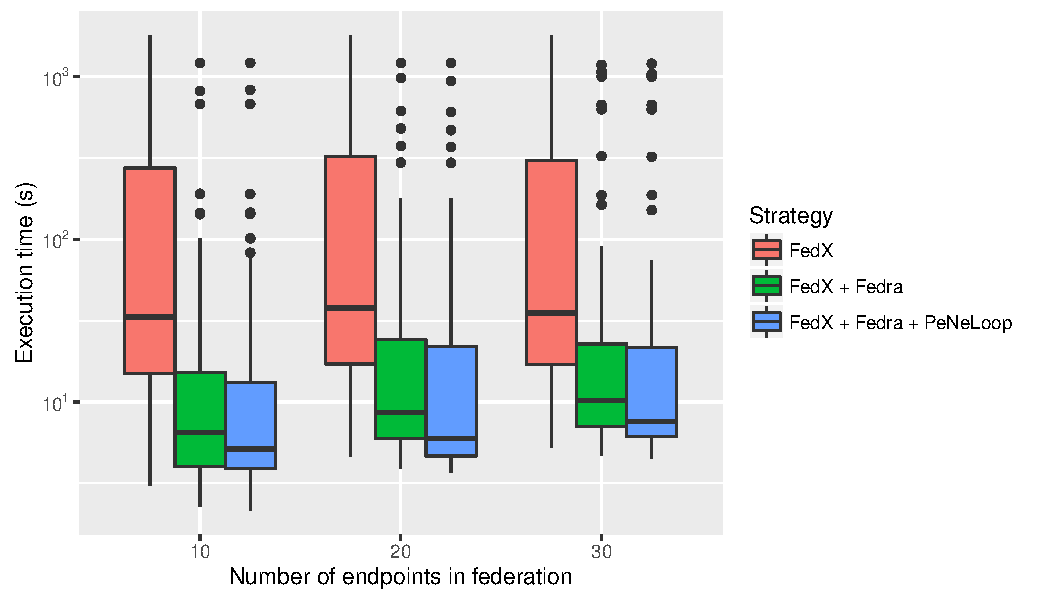
\includegraphics{boxplots/avg_execution_time.pdf}
    \caption{Moyenne des temps d'exécution avec \fedx, \fedx + \fedra et \fedx + \fedra + \peneloop en approche pipeline.}
    \label{fig:avg_time}
\end{figure}

\begin{figure}[h]
    \centering
    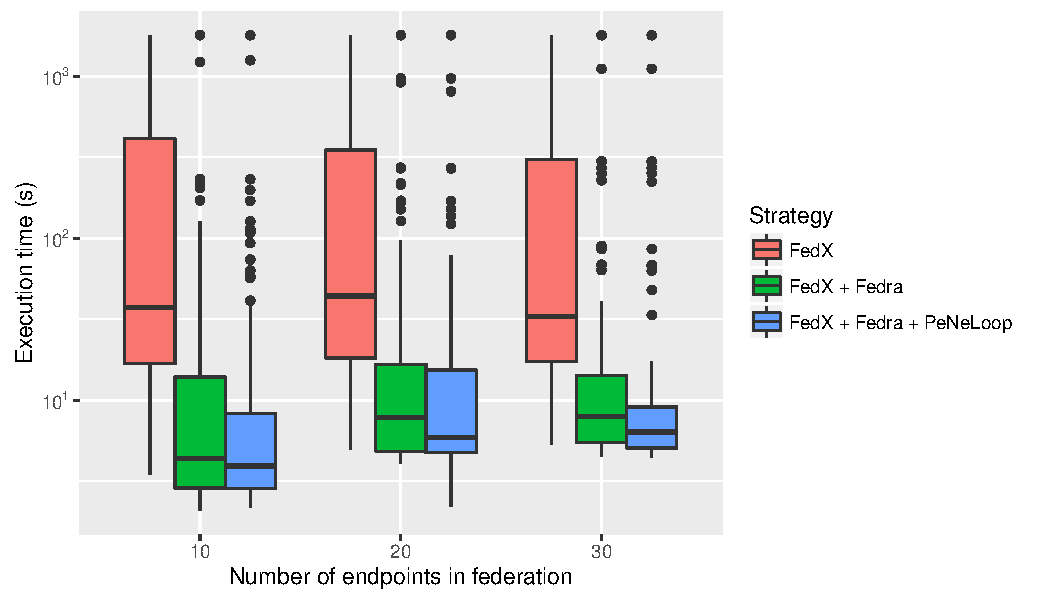
\includegraphics{boxplots/fed1_execution_time.pdf}
    \caption{Temps d'exécution pour le tirage 1 des fédérations avec \fedx, \fedx + \fedra et \fedx + \fedra + \peneloop en approche pipeline. \parallelLink{https://github.com/Callidon/ParallelNestedLoop/blob/master/results/definitive/fed1_pll_execution_time.pdf}}
    \label{fig:fed1_time}
\end{figure}

\begin{figure}[h]
    \centering
    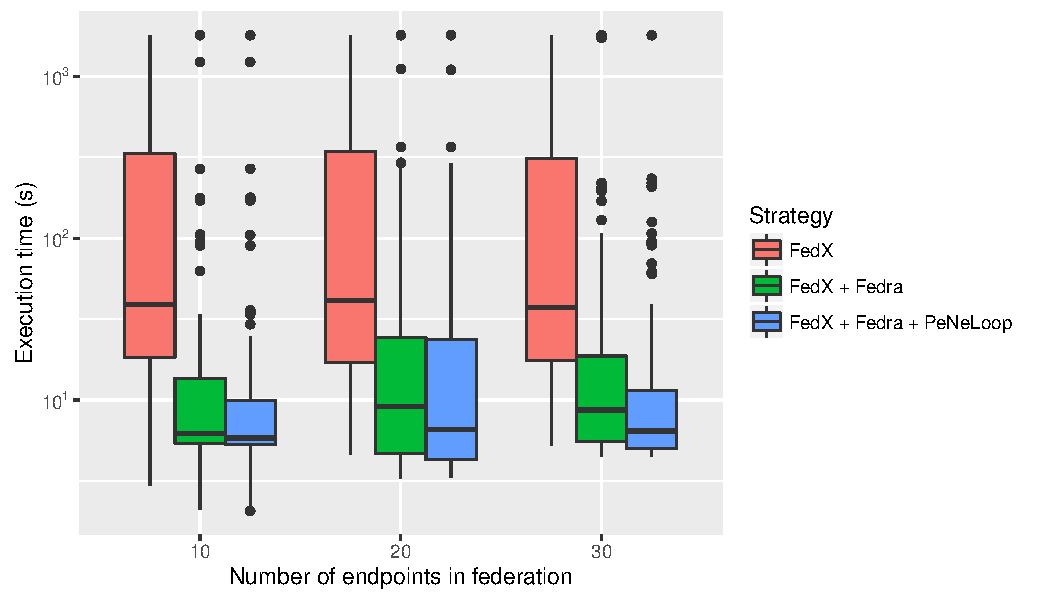
\includegraphics{boxplots/fed2_execution_time.pdf}
    \caption{Temps d'exécution pour le tirage 2 des fédérations avec \fedx, \fedx + \fedra et \fedx + \fedra + \peneloop en approche pipeline. \parallelLink{https://github.com/Callidon/ParallelNestedLoop/blob/master/results/definitive/fed2_pll_execution_time.pdf}}
    \label{fig:fed2_time}
\end{figure}

\begin{figure}[h]
    \centering
    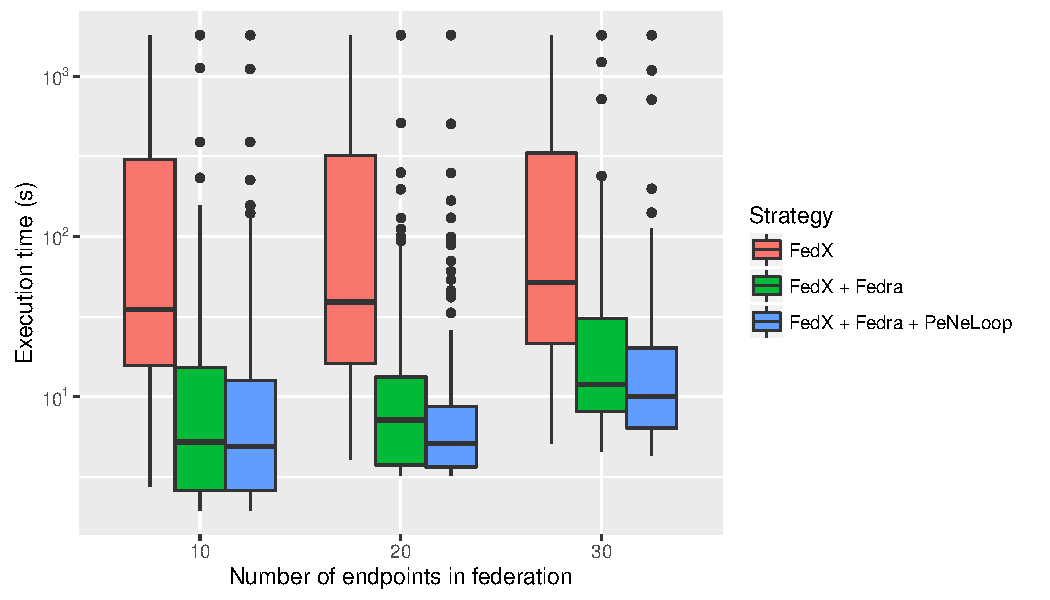
\includegraphics{boxplots/fed3_execution_time.pdf}
    \caption{Temps d'exécution pour le tirage 3 des fédérations avec \fedx, \fedx + \fedra et \fedx + \fedra + \peneloop en approche pipeline. \parallelLink{https://github.com/Callidon/ParallelNestedLoop/blob/master/results/definitive/fed3_pll_execution_time.pdf}}
    \label{fig:fed3_time}
\end{figure}

\begin{figure}[h]
    \centering
    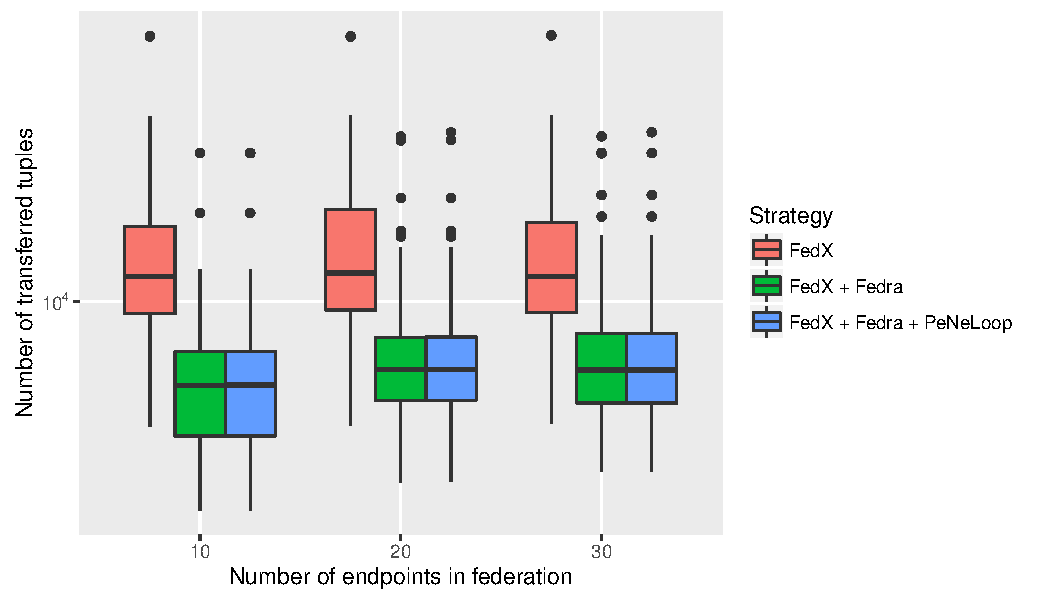
\includegraphics{boxplots/avg_transferred_tuples.pdf}
    \caption{Moyenne du nombre de tuples transférés avec \fedx, \fedx + \fedra et \fedx + \fedra + \peneloop en approche pipeline.}
    \label{fig:avg_tuples}
\end{figure}

\begin{figure}[h]
    \centering
    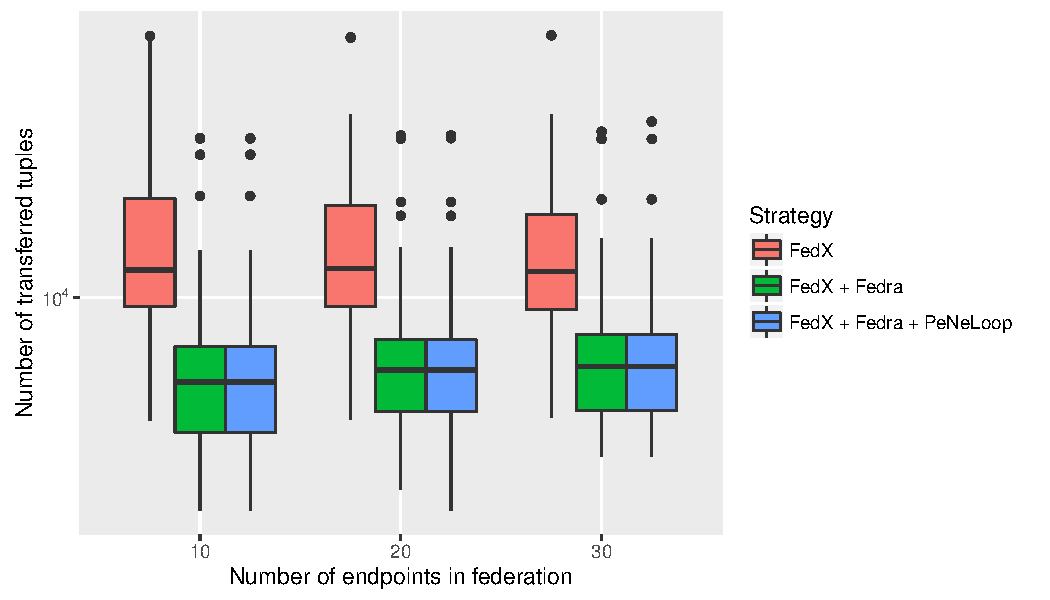
\includegraphics{boxplots/fed1_transferred_tuples.pdf}
    \caption{Nombre de tuples transférés pour le tirage 1 des fédérations avec \fedx, \fedx + \fedra et \fedx + \fedra + \peneloop en approche pipeline. \parallelLink{https://github.com/Callidon/ParallelNestedLoop/blob/master/results/definitive/fed1_pll_transferred_tuples.pdf}}
    \label{fig:fed1_tuples}
\end{figure}

\begin{figure}[h]
    \centering
    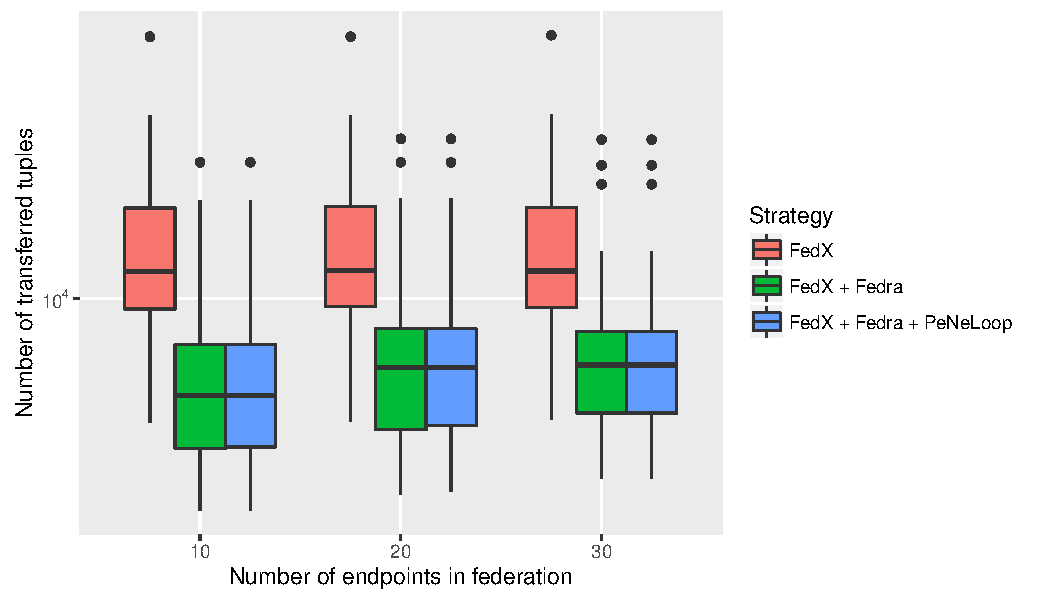
\includegraphics{boxplots/fed2_transferred_tuples.pdf}
    \caption{Nombre de tuples transférés pour le tirage 2 des fédérations avec \fedx, \fedx + \fedra et \fedx + \fedra + \peneloop en approche pipeline. \parallelLink{https://github.com/Callidon/ParallelNestedLoop/blob/master/results/definitive/fed2_pll_transferred_tuples.pdf}}
    \label{fig:fed2_tuples}
\end{figure}

\begin{figure}[h]
    \centering
    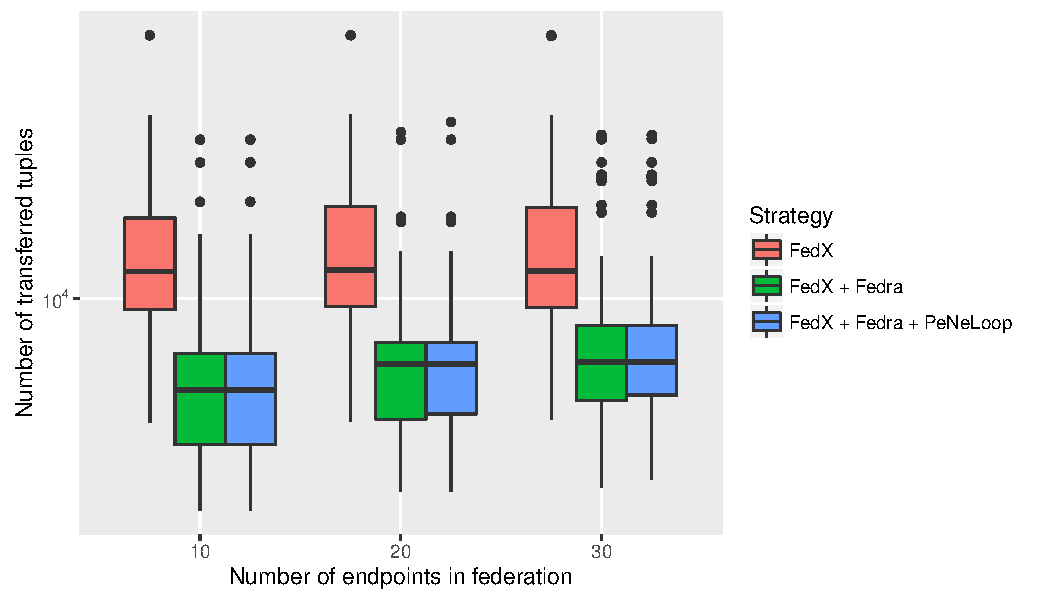
\includegraphics{boxplots/fed3_transferred_tuples.pdf}
    \caption{Nombre de tuples transférés pour le tirage 3 des fédérations avec \fedx, \fedx + \fedra et \fedx + \fedra + \peneloop en approche pipeline. \parallelLink{https://github.com/Callidon/ParallelNestedLoop/blob/master/results/definitive/fed3_pll_transferred_tuples.pdf}}
    \label{fig:fed3_tuples}
\end{figure}

\begin{figure}[h]
    \centering
    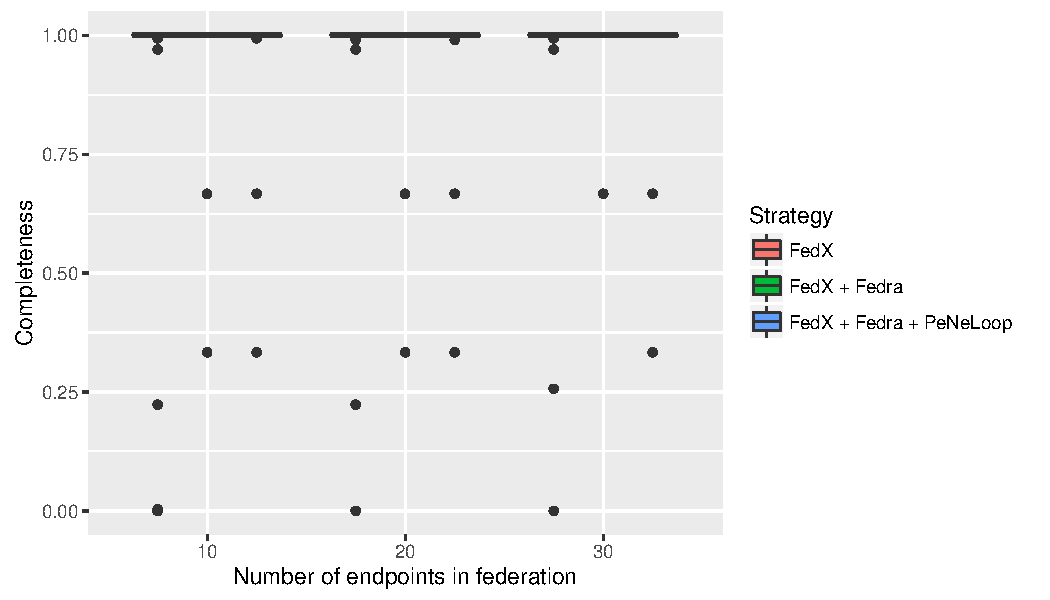
\includegraphics{boxplots/avg_completeness.pdf}
    \caption{Moyenne de la complétude des requêtes pour le tirage 1 des fédérations avec \fedx, \fedx + \fedra et \fedx + \fedra + \peneloop en approche pipeline.}
    \label{fig:avg_compl}
\end{figure}

\begin{figure}[h]
    \centering
    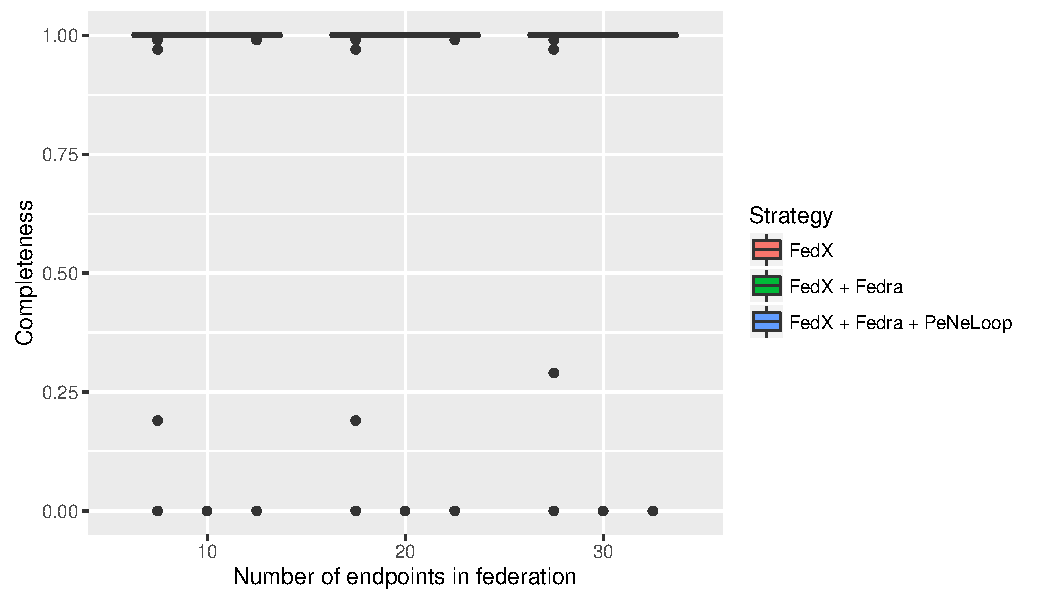
\includegraphics{boxplots/fed1_completeness.pdf}
    \caption{Complétude des requêtes pour le tirage 1 des fédérations avec \fedx, \fedx + \fedra et \fedx + \fedra + \peneloop en approche pipeline. \parallelLink{https://github.com/Callidon/ParallelNestedLoop/blob/master/results/definitive/fed1_pll_completeness.pdf}}
    \label{fig:fed1_compl}
\end{figure}

\begin{figure}[h]
    \centering
    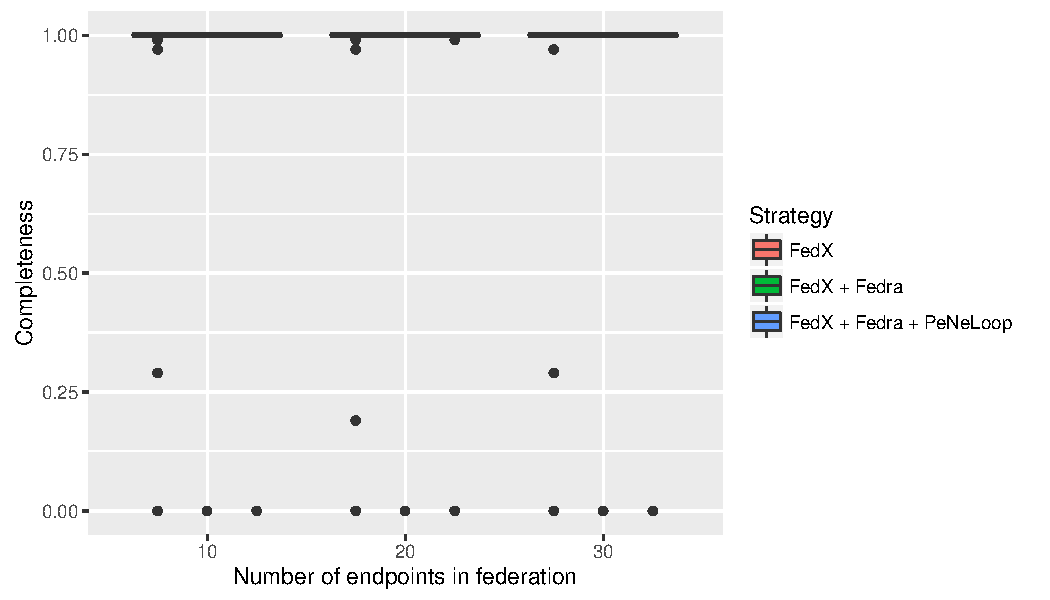
\includegraphics{boxplots/fed2_completeness.pdf}
    \caption{Complétude des requêtes pour le tirage 2 des fédérations avec \fedx, \fedx + \fedra et \fedx + \fedra + \peneloop en approche pipeline. \parallelLink{https://github.com/Callidon/ParallelNestedLoop/blob/master/results/definitive/fed2_pll_completeness.pdf}}
    \label{fig:fed2_compl}
\end{figure}

\begin{figure}[h]
    \centering
    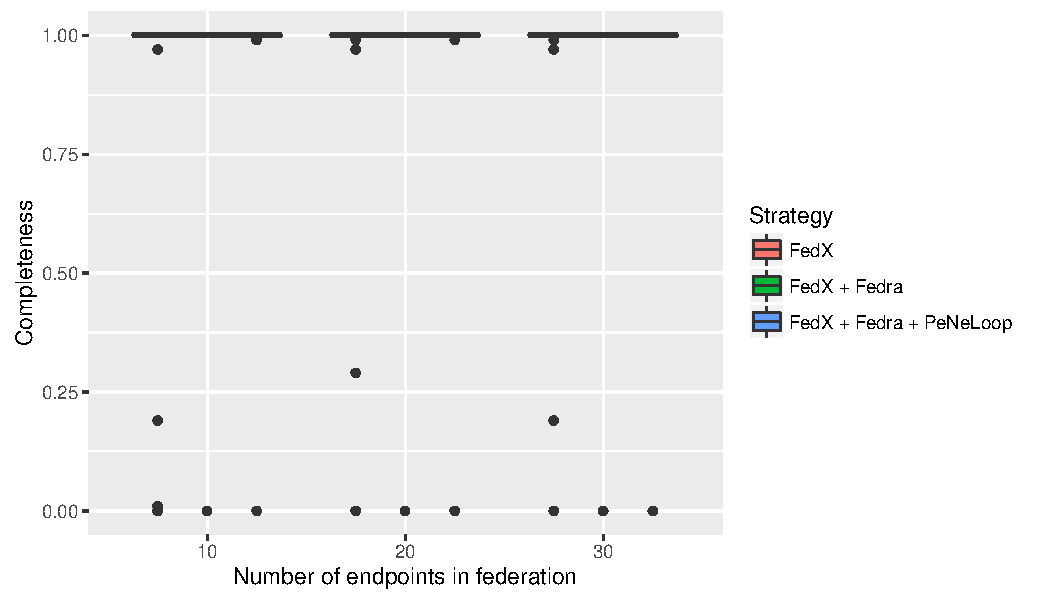
\includegraphics{boxplots/fed3_completeness.pdf}
    \caption{Complétude des requêtes pour le tirage 3 des fédérations avec \fedx, \fedx + \fedra et \fedx + \fedra + \peneloop en approche pipeline. \parallelLink{https://github.com/Callidon/ParallelNestedLoop/blob/master/results/definitive/fed3_pll_completeness.pdf}}
    \label{fig:fed3_compl}
\end{figure}

\end{document}
